\documentclass[a4paper,oneside,12pt]{article}

\usepackage[top=3.0cm,bottom=2.0cm,left=2.9cm,right=2.9cm]{geometry}
\usepackage[portuges]{babel}
\usepackage{amsmath,amsfonts,amssymb}
\usepackage{graphicx,color}
\usepackage{enumerate}
\usepackage{amsmath}
\usepackage{mathtools}
\usepackage{color}
\usepackage{pdfpages}

\begin{document}

\bfseries
\noindent
Universidade Federal do Rio Grande do Norte \\
Programa de P\'os-Gradua\c{c}\~ao em Engenharia El\'etrica e de Computa\c{c}\~ao \\
Redes Neurais (EEC1505) \\
Prof. Adri\~ao Duarte Doria Neto \\
Alunos: Jos\'e Lenival Gomes de Fran\c{c}a, Raphael Diego Comesanha e Silva, Danilo de Santana Pena.
\mdseries

\begin{center}
Lista 3 Exerc\'icios
\end{center}

\begin{enumerate}[1.]
\item A representa\c{c}\~ao de uma determinada mensagem digital tern\'aria, isto \'e formada por tr\^es bits, forma um cubo cujos v\'ertices correspondem a mesma representa\c{c}\~ao digital. Supondo que ao transmitirmos esta mensagem a mesma seja contaminada por ru\'ido formando em torno de cada v\'ertice uma nuvem esf\'erica de valores aleat\'orios. O raio da esfera corresponde ao desvio padr\~ao do sinal de ru\'ido. Solucione o problema usando m\'aquinas de vetor de suporte linear. Compare com a solu\c{c}\~ao obtida na lista 2 onde foi usada uma rede de perceptron de Rosemblat com uma camada para atuar como classificador/decodificador. Para solu\c{c}\~ao do problema defina antes um conjunto de treinamento e um conjunto de valida\c{c}\~ao. \\
%
%RESOLU\c{C}\~AO: \\
%
%... \\

\item Implemente a RBF considerando os algoritmos de treinamento para as tr\^{e}s situa\c{c}\~oes: (a) centros fixos e escolhidos aleatoriamente, (b) centros escolhidos atrav\'es da sele\c{c}\~ao auto-supervisionada (algoritmo K-means) , (c) centros escolhidos atrav\'es da sele\c{c}\~ao supervisionada, para as tr\^es quest\~oes abaixo: \\

\begin{enumerate}[a)]
\item A fun\c{c}\~ao l\'ogica $f(x_{1}, x_{2}, x_{3}) = x_{1} \oplus x_{2} \oplus x_{3}$

\item \begin{equation*}
f(x) = \left[ \frac{sin(\pi ||x||)}{\pi ||x||} \right] \text{, } x = \begin{bmatrix}
x_{1} \\
x_{2}
\end{bmatrix} \text{, } |x_{1}| \leq 10 \text{ e } |x_{2}| \leq 10
\end{equation*}

\item $f(x) = x_{1}^{2} + x_{2}^{2} - 2 x_{1} x_{2} + x_{1} + x_{2} - 1$, $|x_{1}| \leq 10$, $|x_{2}| \leq 10$
\end{enumerate}

RESOLU\c{C}\~AO: \\

As alternativas $a)$ e $c)$ possuiram erro igual a $0$. Na alternativa $b)$ n\~ao conseguiu-se bons resultados utilizando a $toolbox$, pois a sa\'ida da rede resulta em valor $NaN$.

Segue o c\'odigo utilizando a \emph{toolbox} do MATLAB:

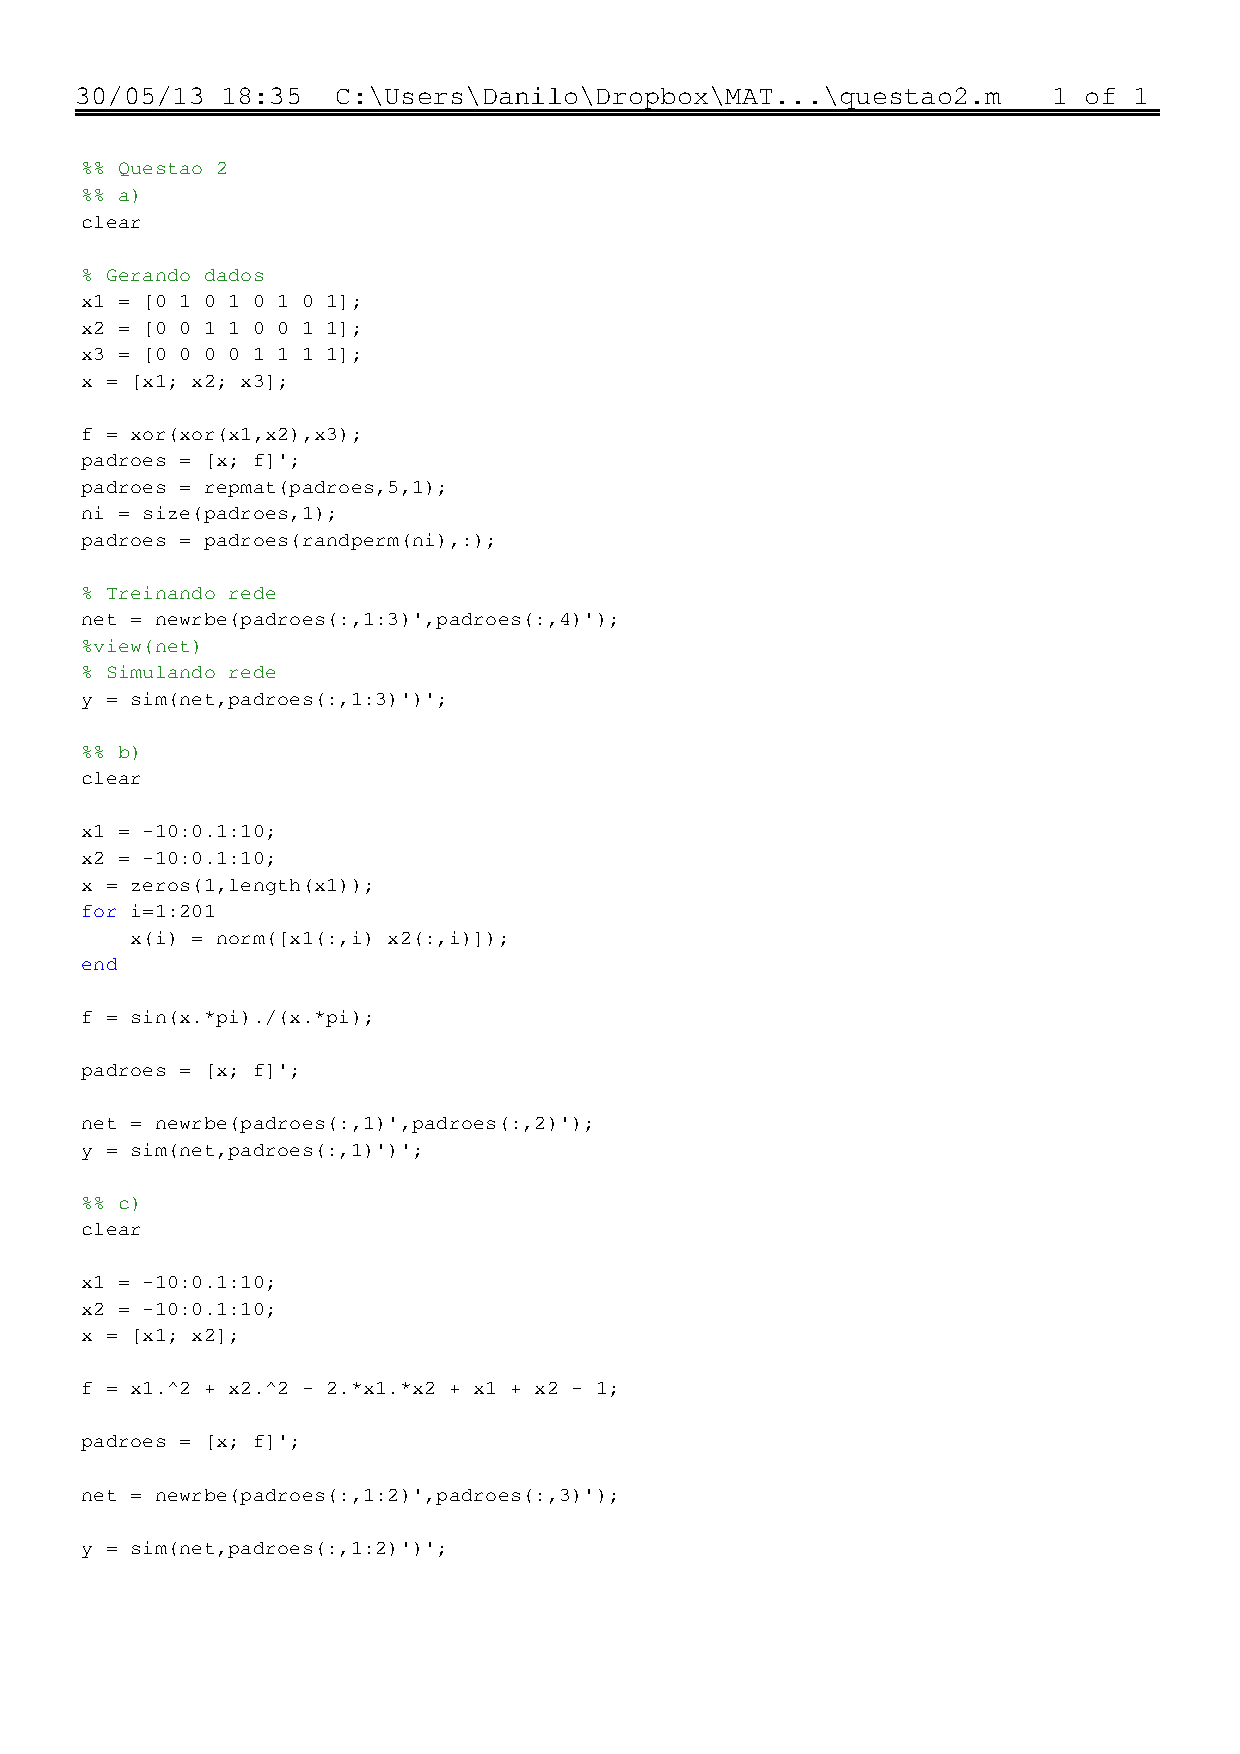
\includepdf[pages=-]{q2.pdf}

\item Considere o problema de classifica\c{c}\~ao de padr\~oes constitu\'ido neste caso de 12 padr\~oes. A distribui\c{c}\~ao dos padr\~oes tem como base um quadrado centrado no ponto (0.5,0.5) e lados iguais a 1. Os pontos (0.5,0.5), (1.0,0.5), (0.5,1.) e (0.0, 0.5) s\~ao centros de quatro semic\'irculos que se interceptam no interior do quadrado originando quatro classes e outras oito classes nas regi\~oes de n\~ao interse\c{c}\~ao. Ap\'os gerar aleatoriamente dados que venham formar estas distribui\c{c}\~oes de dados, selecione um conjunto de treinamento e um conjunto de valida\c{c}\~ao. Solucione o problema usando RBF, SVM e M\'aquina de Comit\^e. Verifique o desempenho do classificador usando o conjunto de valida\c{c}\~ao e calculando a matriz de confus\~ao e compare com o obtido na lista anterior usando MLP. \\

RESOLU\c{C}\~AO: \\

Segue abaixo nossa implementa\c{c}\~ao da RBF, com problema para convergir (apenas converge para erro igual zero ap\'os algumas tentativas).

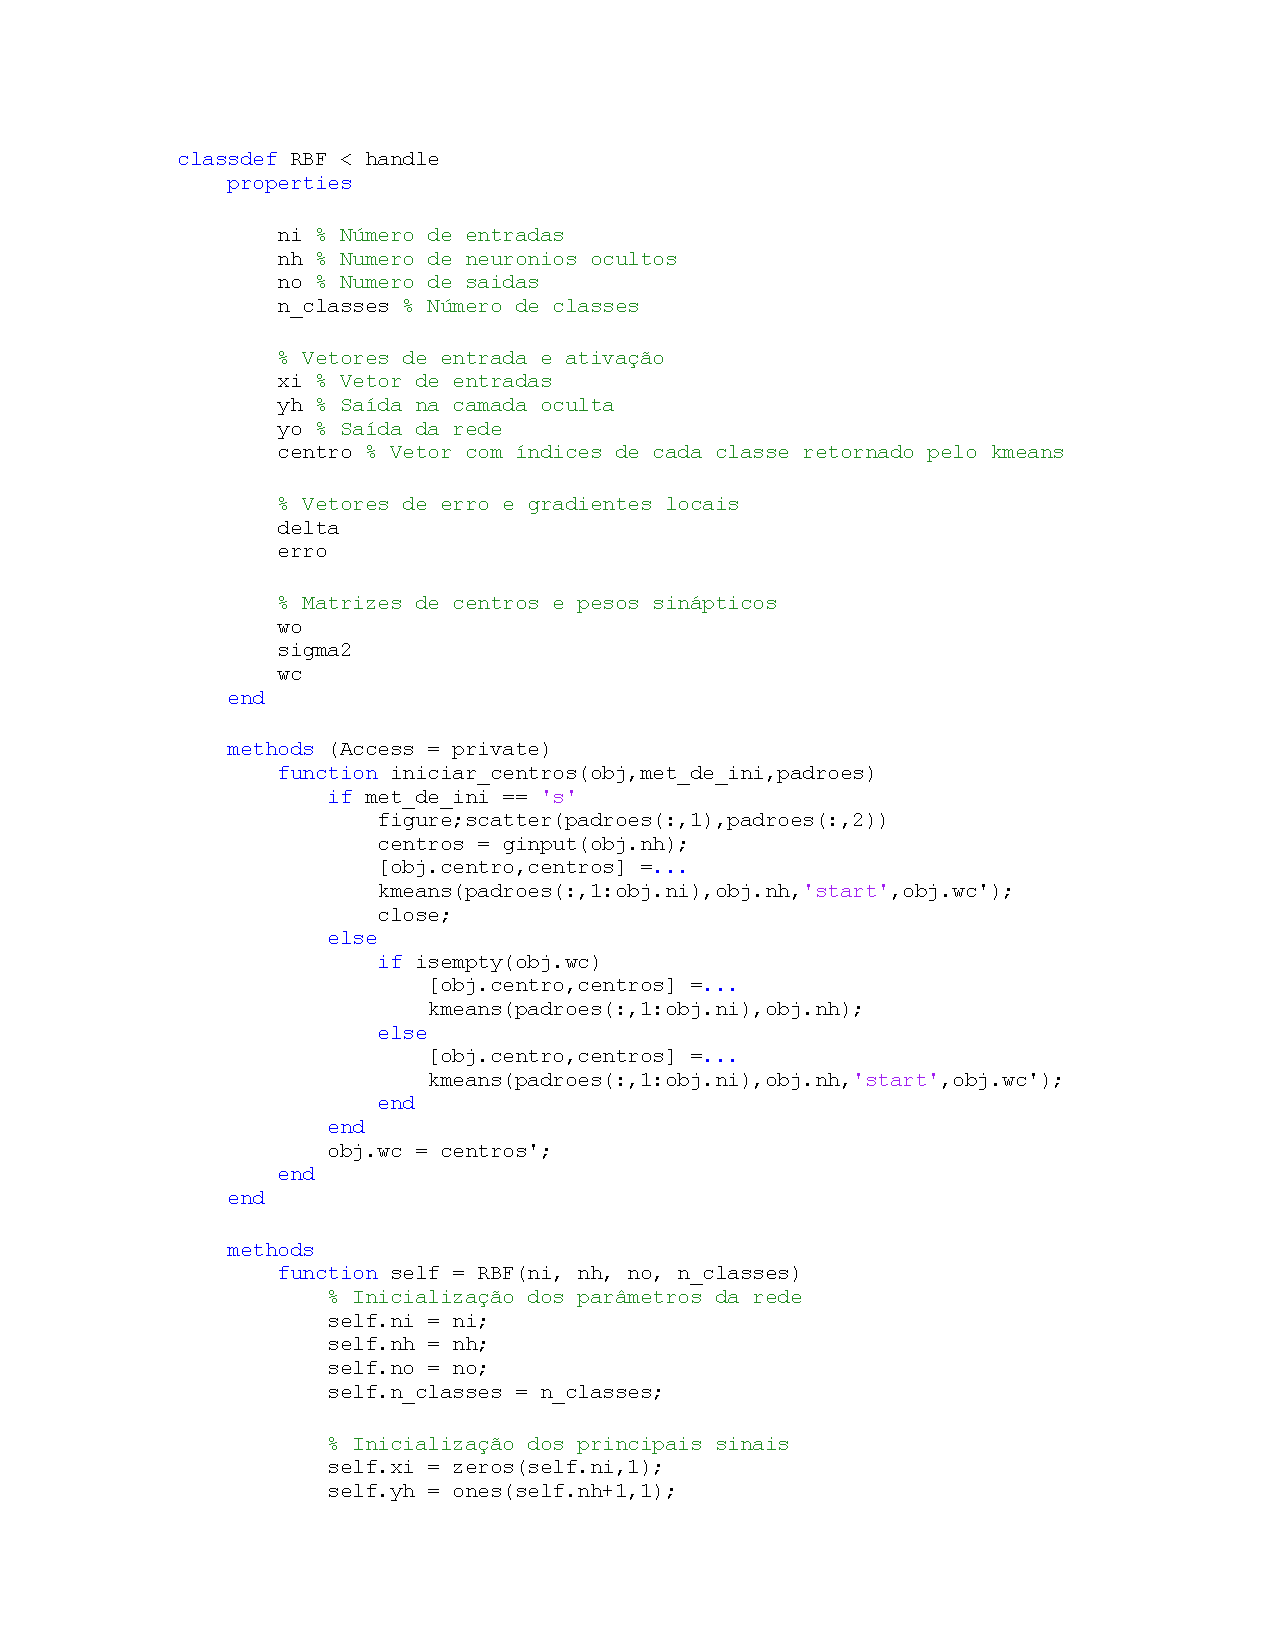
\includepdf[pages=-]{q3.pdf}

\item Utilize uma rede NARX, no caso uma rede neural perceptron de m\'ultiplas camadas com realimenta\c{c}\~ao global, para fazer a predi\c{c}\~ao de um passo, at\'e predi\c{c}\~ao de tr\^es passos da s\'erie temporal $x(n) = 1 + cos(n + cos 2 (n))$. Avalie o desempenho mostrando para cada caso os erros de predi\c{c}\~ao. \\

RESOLU\c{C}\~AO: \\

Foi utilizado a \emph{toolbox} do MATLAB, como segue nas figuras \ref{fig:q4_1} e \ref{fig:q4_2}. O c\'odigo segue abaixo:

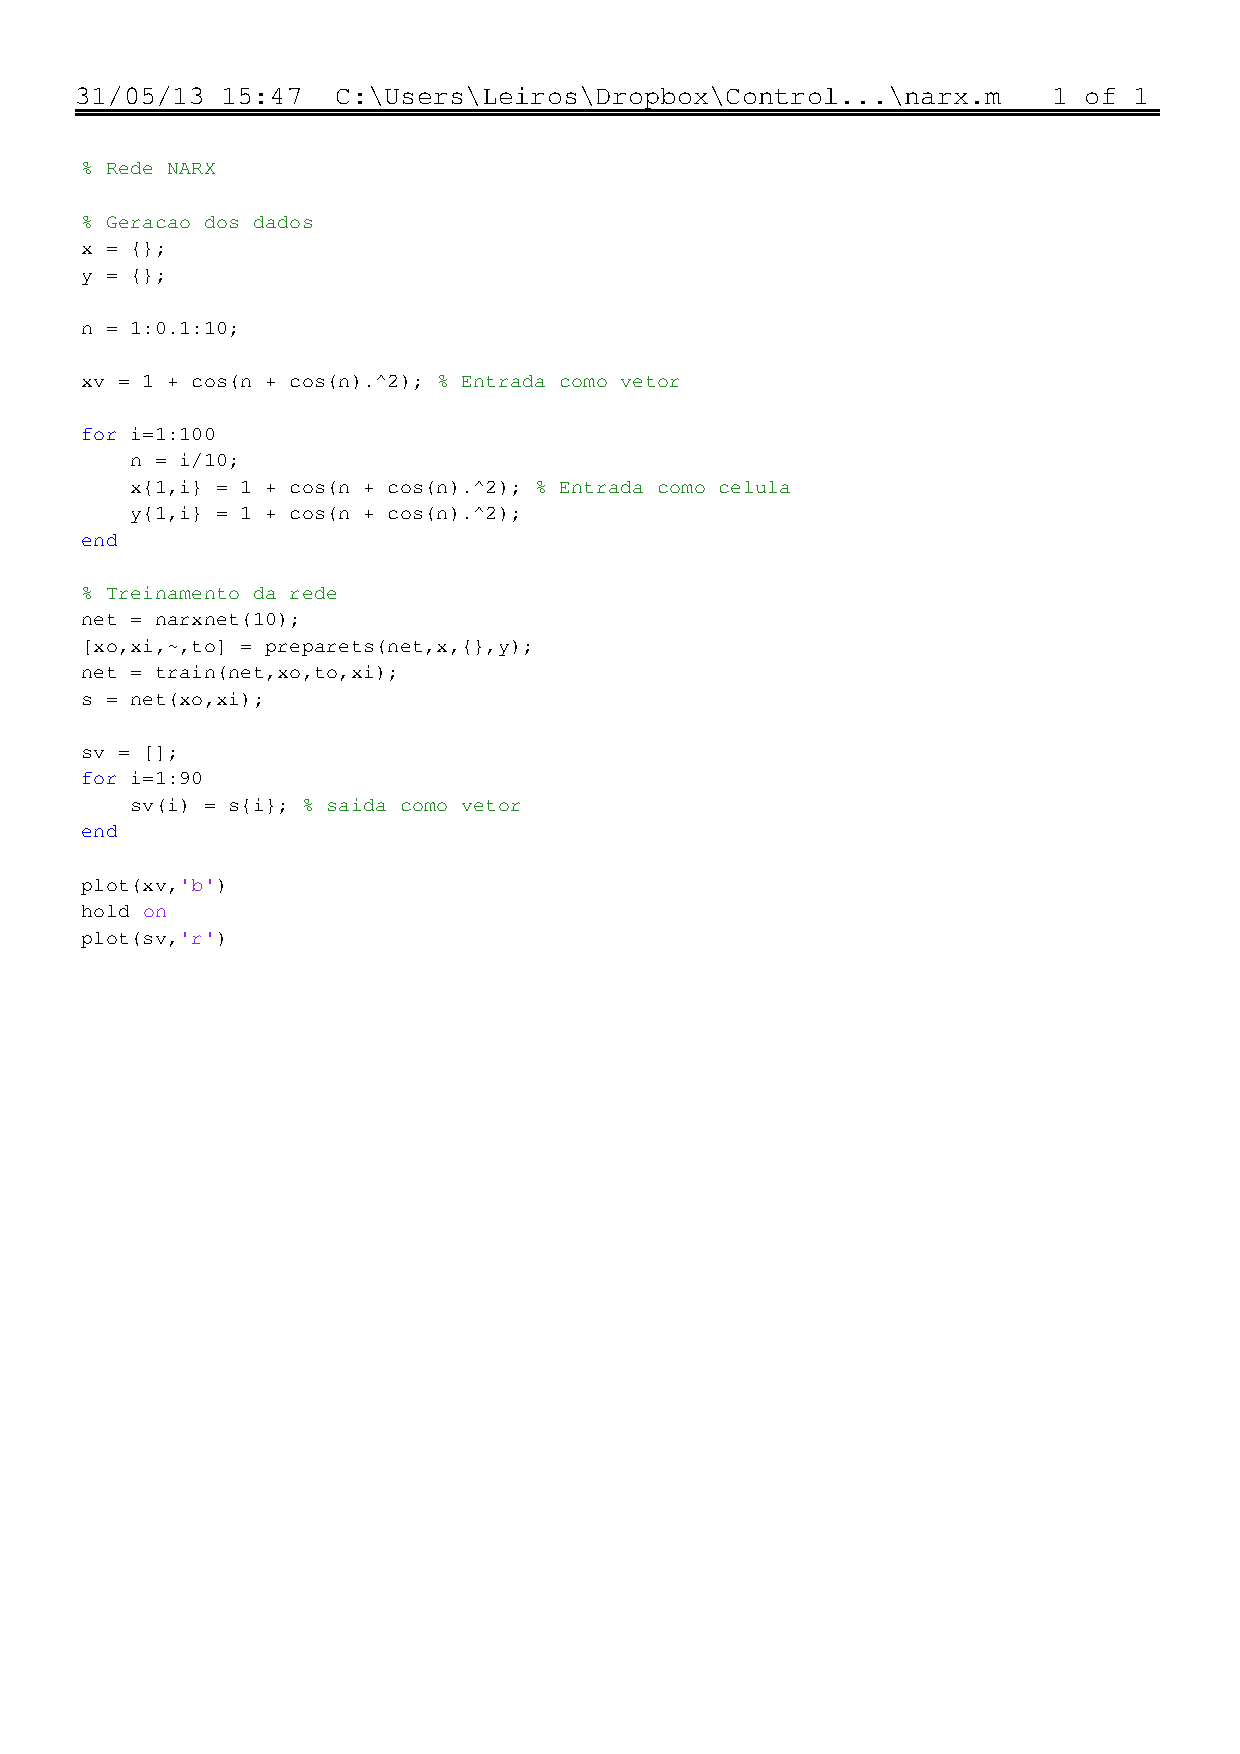
\includepdf[pages=-]{q4.pdf}

\begin{figure}[h!]
\centering
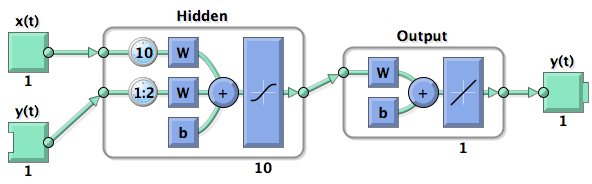
\includegraphics[width=0.8\textwidth]{q4_1.png}
\caption{Arquitetura da rede NARX utiizada.}
\label{fig:q4_1}
\end{figure}

\begin{figure}[h!]
\centering
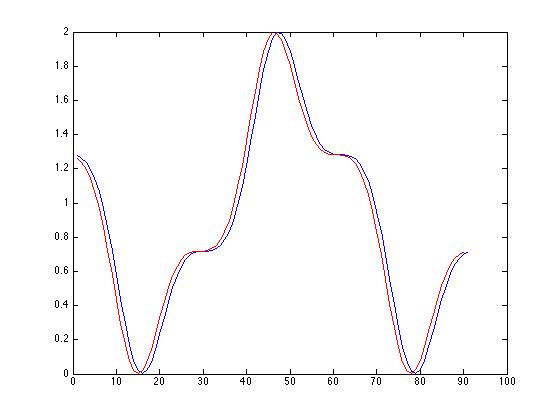
\includegraphics[width=0.8\textwidth]{q4_2.png}
\caption{Resultado da rede NARX.}
\label{fig:q4_2}
\end{figure}

\item Implemente uma rede de Hopfield, para reconhecer as letras AFC. (Para cada letra forme uma matriz bin\'aria de pixel). Verifique o desempenho com as letras sendo apresentadas de forma ruidosa. \\

RESOLU\c{C}\~AO: \\

A implementa\c{c}\~ao da rede Hopfield \'e feita como segue:

\begin{equation*}
u_{j}(k) = \sum_{i=1}^{n} W_{ji} \cdot v_{i}(k-1) + i_{j}^{b} \text{, onde } j = 1, \cdots, n
\end{equation*}

\begin{equation*}
v_{j}(k) = g(u_{j}(k))
\end{equation*}

onde $k$ \'e um passo de itera\c{c}\~ao.

Para garantir a estabilidade da rede, segue-se o algoritmo:

\begin{enumerate}[1)]
\item Especificar a matriz de pesos $W$ e o vetor de limiares $i^b$;

\item Apresentar vetor inicial de entradas ($ x^{(0)} $);

\item $v^{atual} \gets x^{(0)}$;

\item Repetir as instru\c{c}\~oes:

$v^{anterior} \gets v^{atua}$;

$u \gets W \cdot v^{anterior} + i ^{b}$;

$v^{atual} \gets g(u)$;

At\'e que: $v^{atual} \cong v^{anterior}$

\item $v^{final} \gets v^{atual}$ ($v^{final}$ representa um ponto de equil\'ibrio)

\end{enumerate}

\item Dado o modelo n\~ao linear de espa\c{c}o de estado abaixo, obtenha o modelo de espa\c{c}o de estados linearizado para ser utilizado no algoritmo EKF. \\

\begin{equation*}
x(n+1) = f(n, x(n)) + v_{1}(n)
\end{equation*}

\begin{equation*}
y(n) = c(n, x(n)) + v_{2}(n)
\end{equation*}

\begin{equation*}
f(n, x(n)) = \begin{bmatrix}
x_{1}(n) + x_{2}^{2}(n) \\
nx_{1}(n) - x_{1}(n)x_{2}(n)
\end{bmatrix}
\end{equation*}

\begin{equation*}
c(n, x(n)) = x_{1}(n)x_{2}^{2}(n) + v_{2}(n)
\end{equation*}

RESOLU\c{C}\~AO: \\

Foi implementado o EKF como segue abaixo, por\'em para validar o c\'odigo foi utilizado uma outra fun\c{c}\~ao dada por:

\begin{equation*}
f(x(n)) = \begin{bmatrix}
x_{2}(n) \\
x_{3}(n) \\
0.05\cdot x_{1}(n) \cdot (x_{2}(n) + x_{3}(n))
\end{bmatrix}
\end{equation*}

Os resultados est\~ao na figura \ref{fig:q6}.

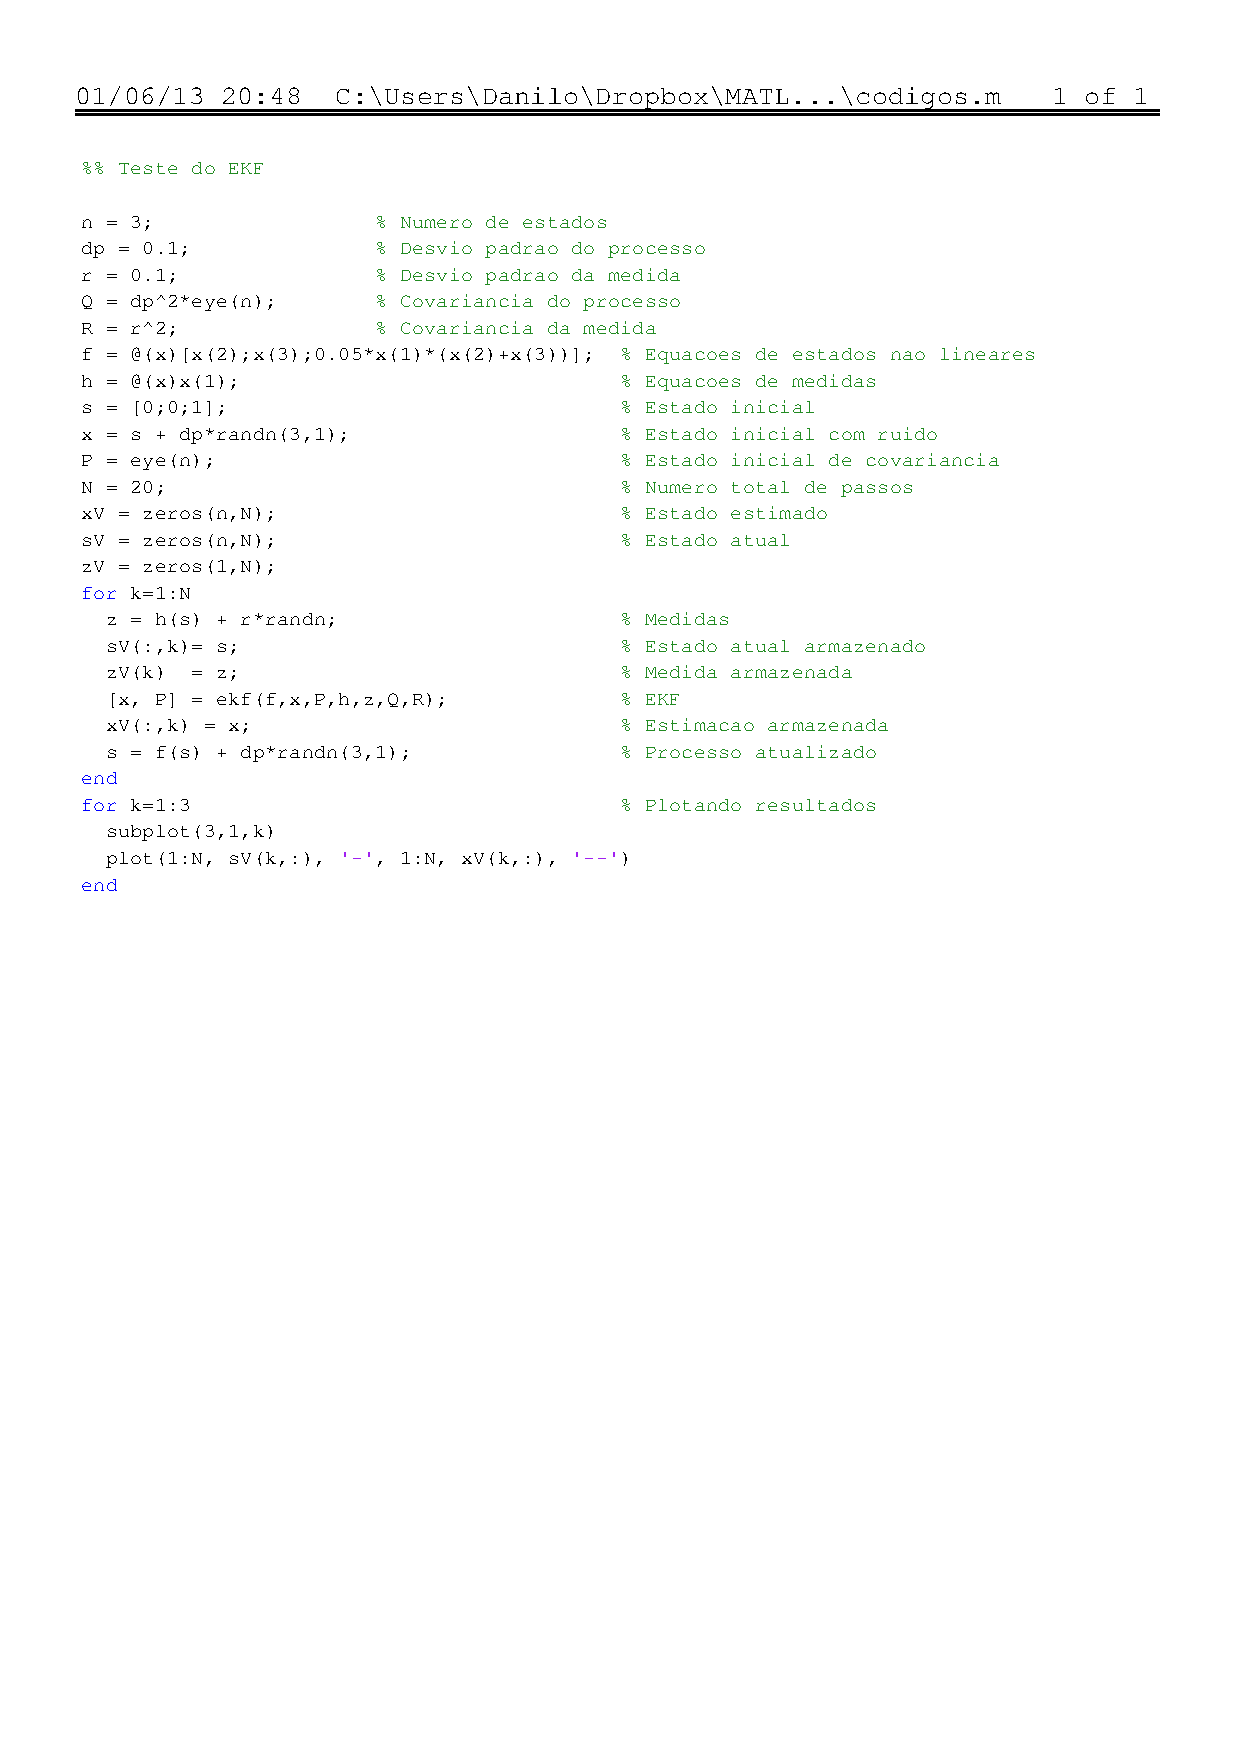
\includepdf[pages=-]{q6_1.pdf}

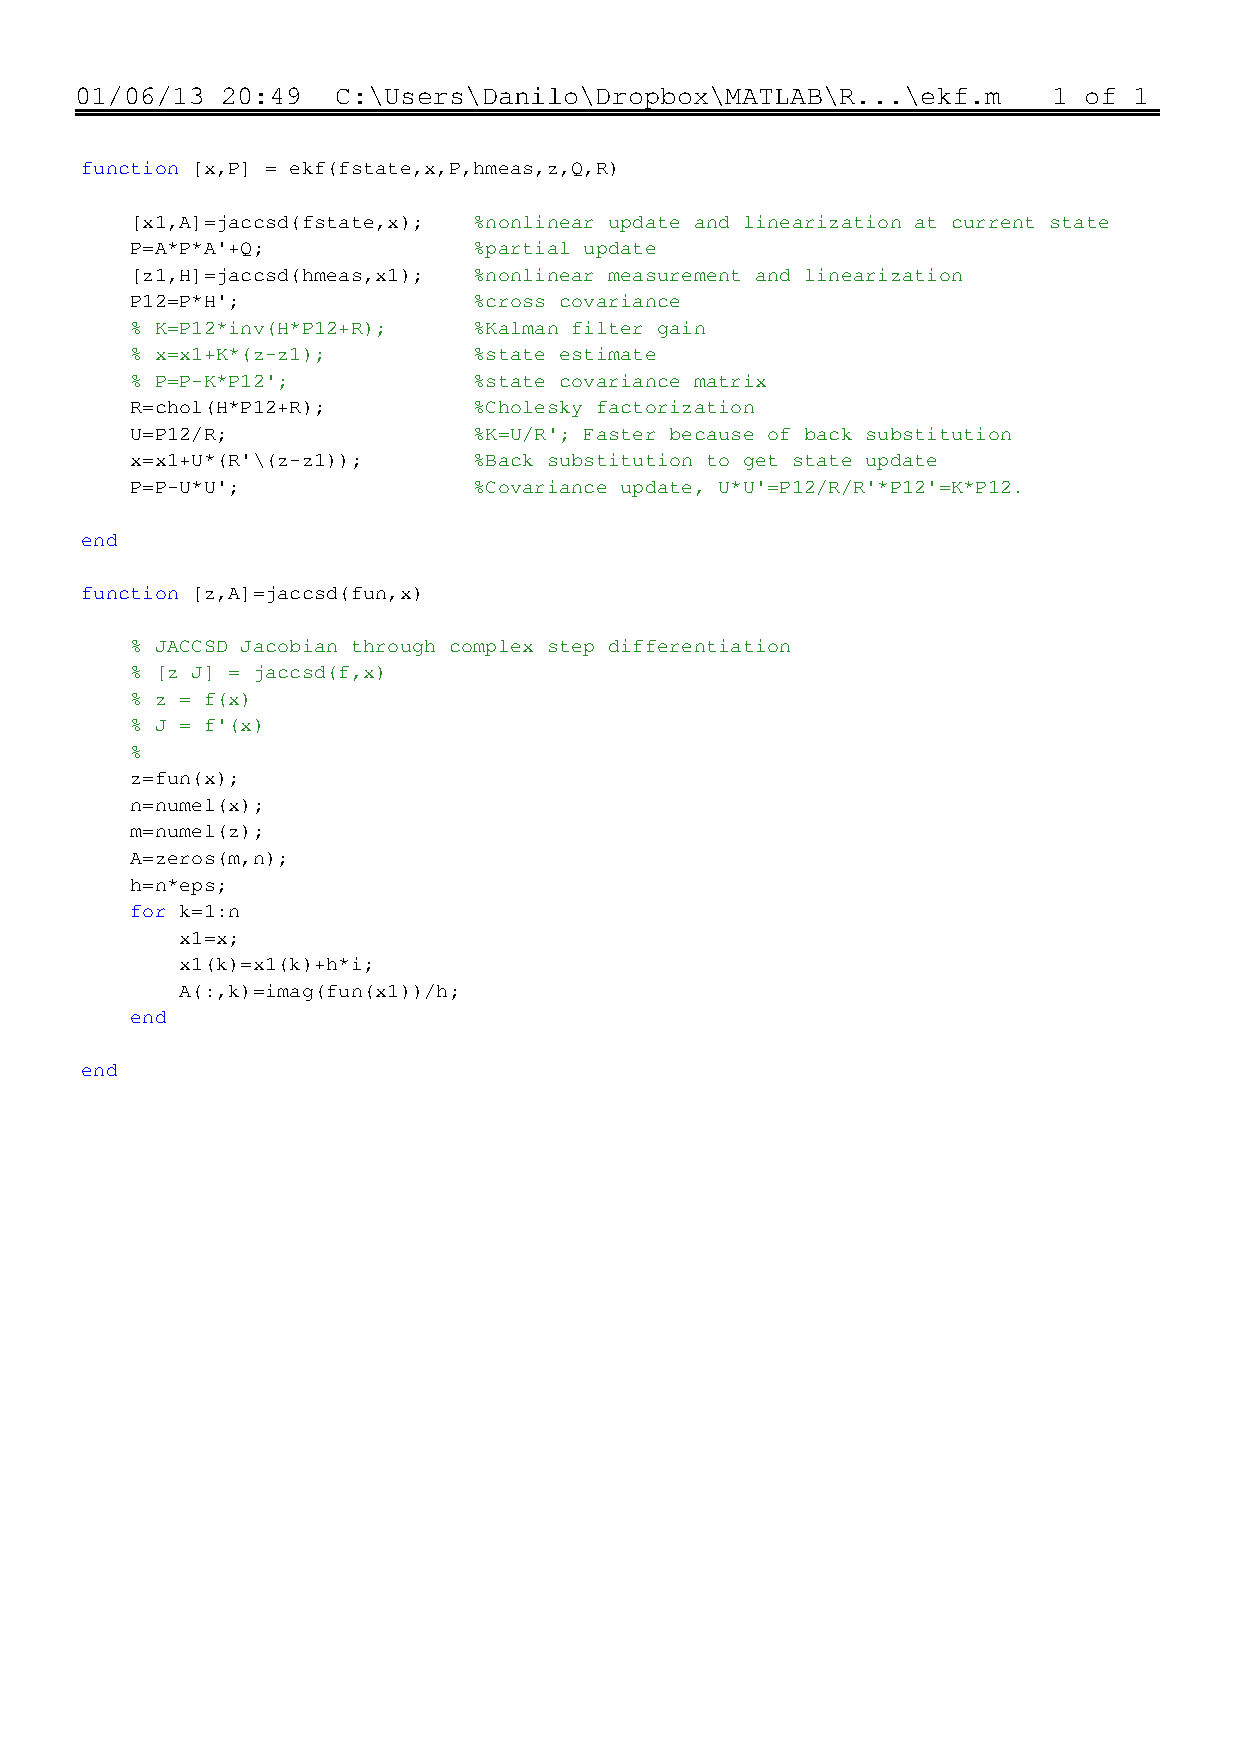
\includepdf[pages=-]{q6_2.pdf}

\begin{figure}[h!]
\centering
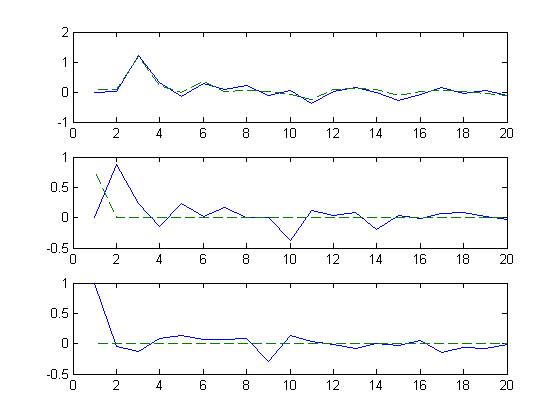
\includegraphics[width=0.8\textwidth]{q6.png}
\caption{Resultado da EKF.}
\label{fig:q6}
\end{figure}

\item Um problema interessante para testar a capacidade de uma rede neural atuar como classificado de padr\~oes \'e o problema das duas espirais intercaladas. Gere os exemplos de treinamento usando as seguintes equa\c{c}\~oes: \\
para espiral 1 $x = \frac{\theta}{4} cos(\theta)$ , $y = \frac{\theta}{4} sen(\theta)$ , $\theta \geq 0$ \\
para espiral 2 $x = (\frac{\theta}{4} + 0.8) cos(\theta)$ , $y = (\frac{\theta}{4} + 0.8) sen(\theta)$ , $\theta \geq 0$ \\
fazendo $\theta$ assumir 51 igualmente espa\c{c}ados valores entre 0 e 20 radianos. Utilize uma rede competitiva e em seguida uma rede SOM para atuar como classificador auto-supervisionado, isto \'e, a espiral 1 sendo uma classe e espiral 2 sendo outra classe. Para comparar as regi\~oes de decis\~oes formadas pela rede , gere uma grade uniforme com 100 x 100 exemplos de teste em um quadrado [-5,5]. Esboce os pontos classificados pela rede. \\

RESOLU\c{C}\~AO: \\

Foram implementados o algoritmo competitivo e o algoritmo SOM, como segue abaixo junto com a especifica\c{c}\~ao:

A execu\c{c}\~ao do algoritmo competitivo para classificar os dados da expiral (classe 1) e da expiral 2 (classe 2) foi definida com as seguintes especifica\c{c}\~oes:

Nº de neur\^onios: 100 \\
Nº de \'epocas: 5000 \\
Taxa de aprendizagem: 0,1 \\
Nº de entradas: 2 \\

Os pesos (representados pelos c\'irculos vermelhos) foram inicializados aleatoriamente em um espa\c{c}o tridimensional normalizado, como mostrado na figura \ref{fig:q7_1}.

\begin{figure}[h]
\centering
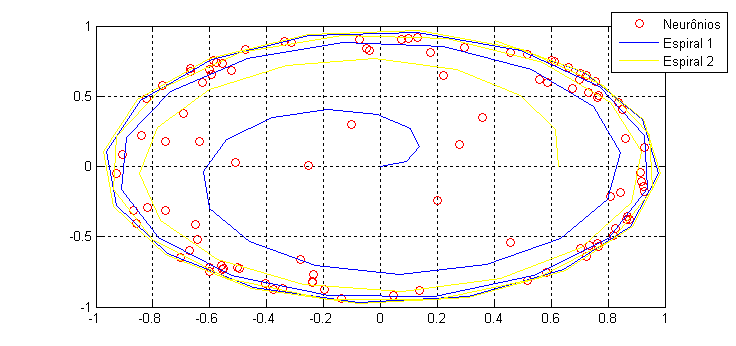
\includegraphics[width=0.8\textwidth]{q7_1.png}
\caption{Resultado da rede SOM para a espiral.}
\label{fig:q7_1}
\end{figure}

Nessa figura \'e poss\'ivel perceber que poucos pesos encontram-se alinhados as espirais.
Ap\'os o treinamento do algoritmo competitivo, os pesos foram deslocados, de tal forma a alinharem-se \`as espirais com ocorr\^encia de poucos pesos desalinhados, como pode ser visto na figura \ref{fig:q7_2}.

\begin{figure}[h]
\centering
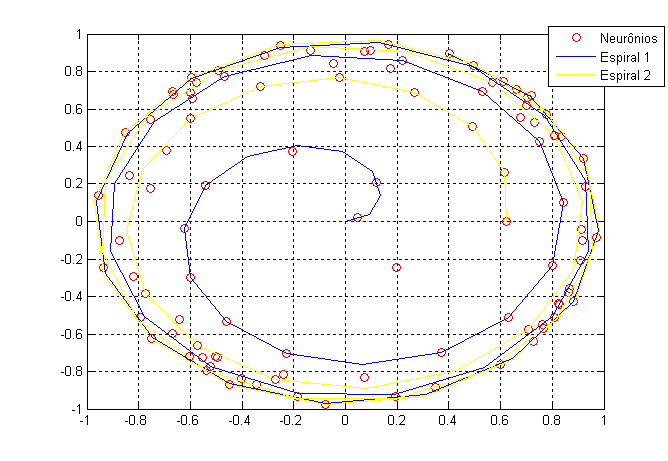
\includegraphics[width=0.8\textwidth]{q7_2.png}
\caption{Resultado da rede SOM para a espiral alinhado.}
\label{fig:q7_2}
\end{figure}

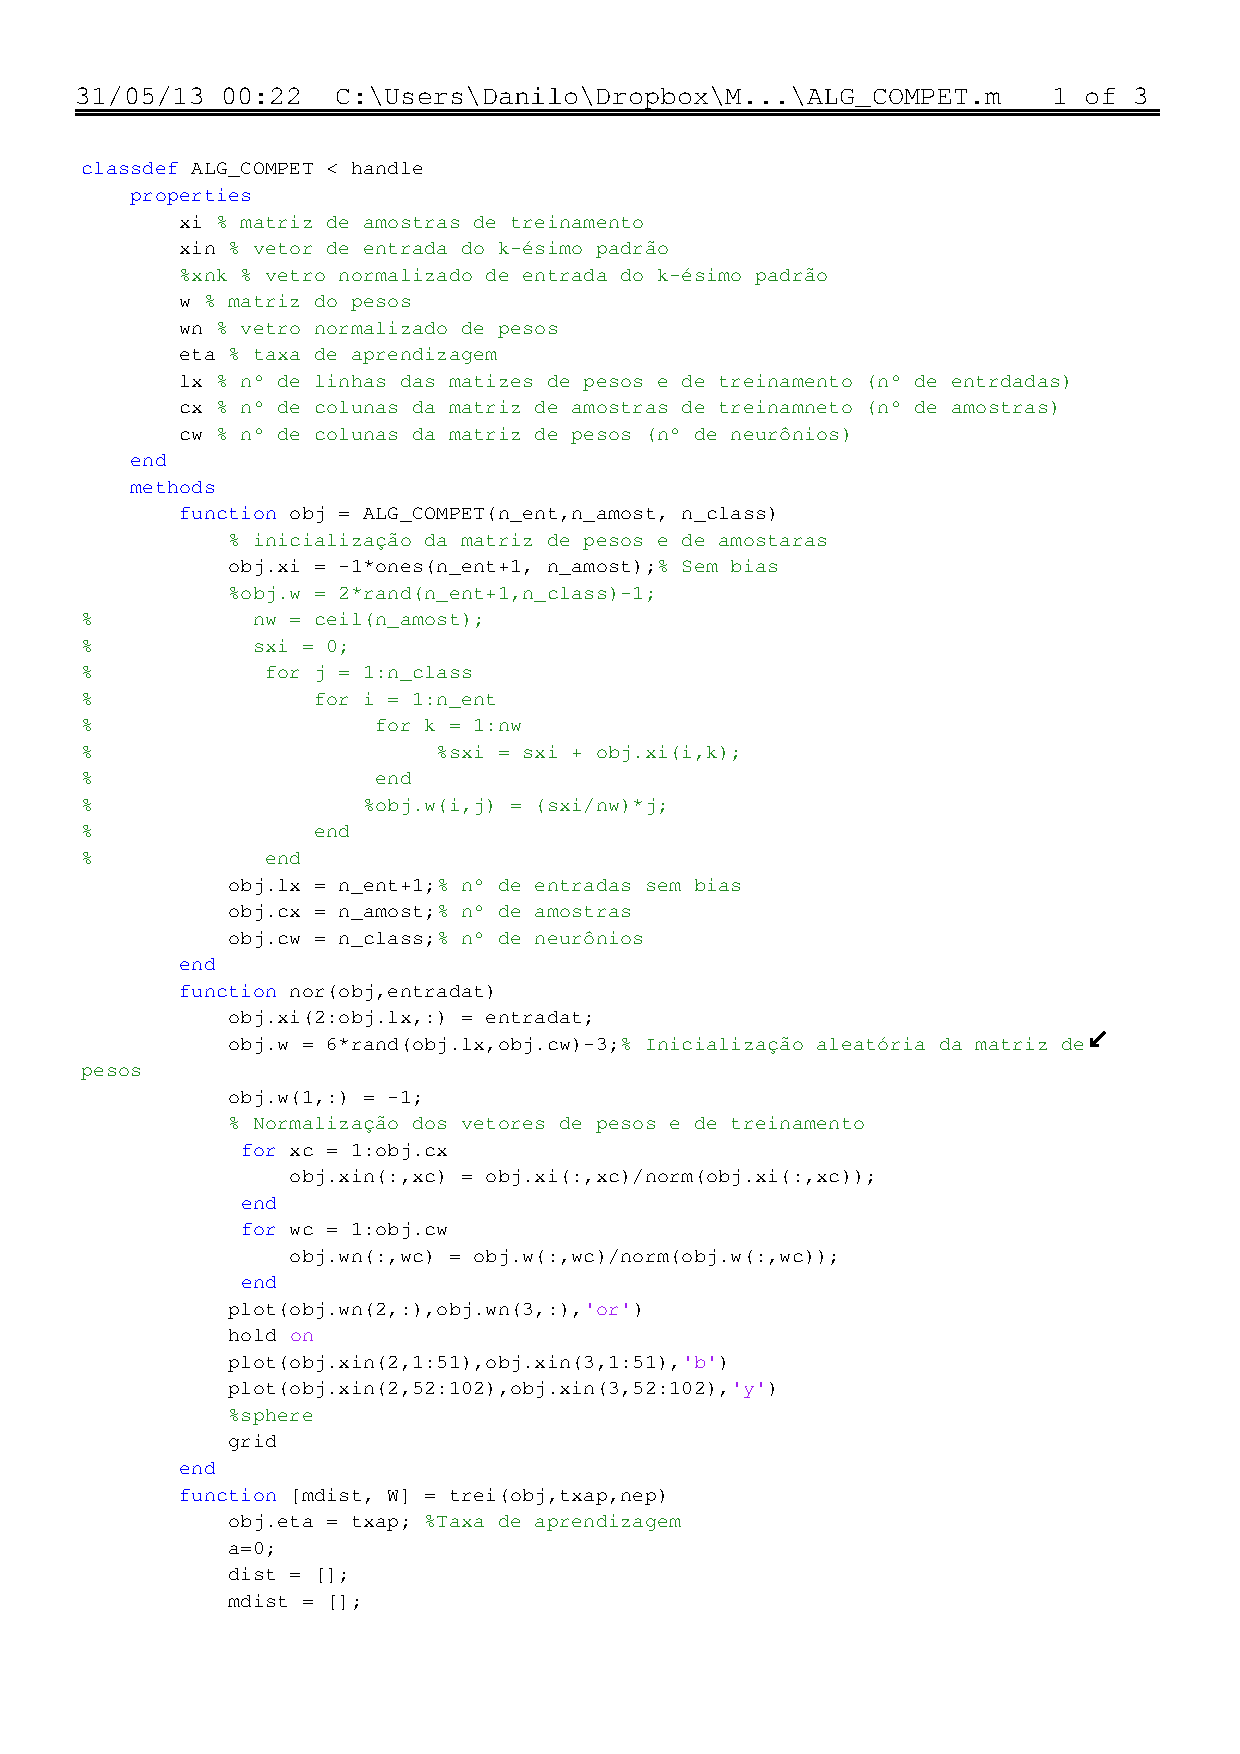
\includepdf[pages=-]{q7_1.pdf}

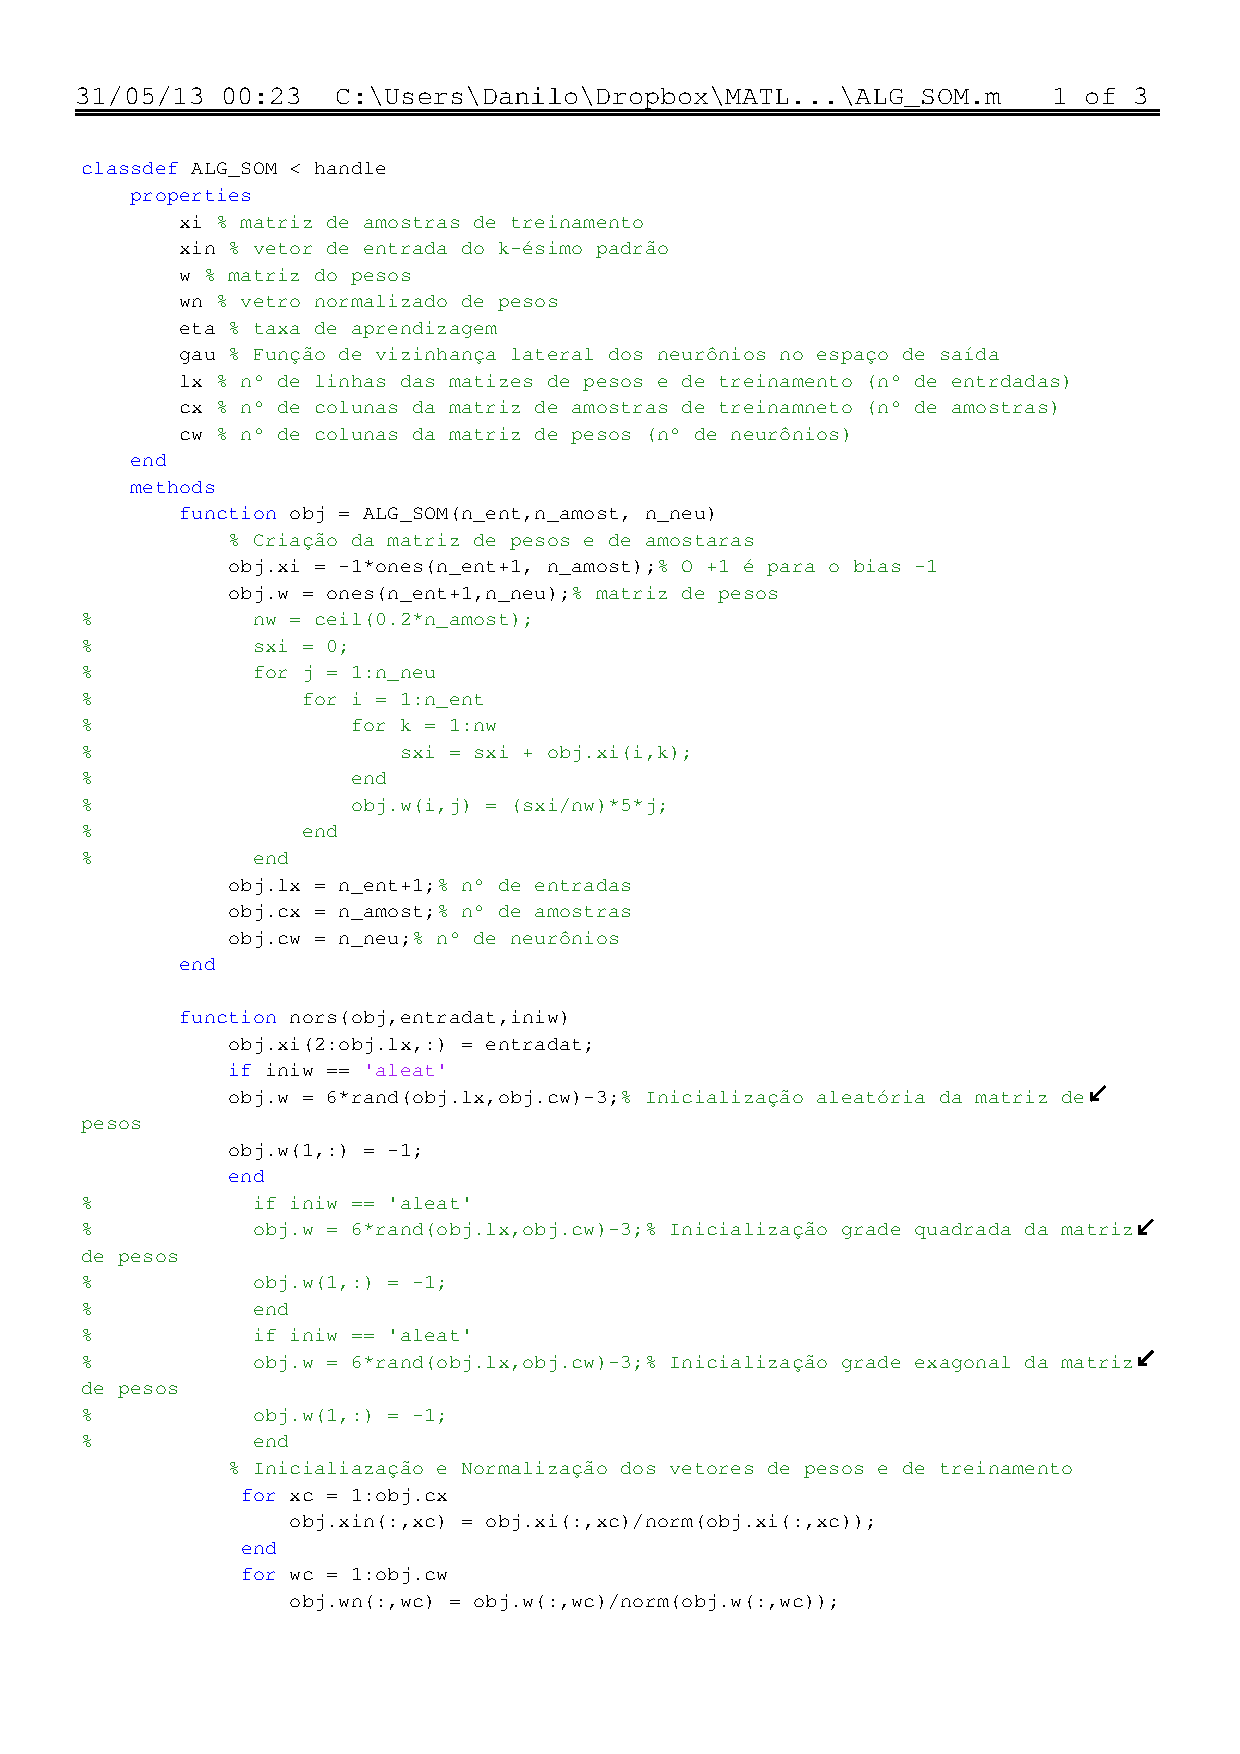
\includepdf[pages=-]{q7_2.pdf}

\item Considere a distribui\c{c}\~ao dos padr\~oes que tem como base em um c\'irculo com raio igual a 0.25 centrado origem. Os pontos +1 e -1 de cada eixo s\~ao centros de quatro semic\'irculos que se interceptam no interior a as regi\~oes que excluem o c\'irculo de raio igual a 0.25 do quadrado originando quatro classes. Gere aleatoriamente os dados que venham formar estas distribui\c{c}\~oes de dados. Utilize a rede SOM de modo a quantizar atrav\'es da distribui\c{c}\~ao de neur\^onios a distribui\c{c}\~ao dos dados. \\

RESOLU\c{C}\~AO: \\

Foi feito a gera\c{c}\~ao dos dados atrav\'es da equa\c{c}\~ao do c\'irculo:

\begin{equation*}
x = \sqrt{r^{2} - (y - y_{0})^{2}} + x_{0}
\end{equation*}

\begin{equation*}
y = \sqrt{r^{2} - (x - x_{0})^{2}} + y_{0}
\end{equation*}

A classifica\c{c}\~ao dos dados foi feito atrav\'es de um vetor $[QX QY H V]$, em que para cada ponto gerado $QX$ representa um dos dois quadrantes no eixo $X$, podendo assim assumir o valor $0$ ou $1$, o equivalente ocorre para $QY$ no eixo $Y$, $H$ representa se o ponto gerado encontra-se dentro de um semi-c\'irculo horizontal e $V$ para um semi-c\'irculo vertical. Com este vetor \'e poss\'ivel classificar o ponto gerado, visto que se o ponto estiver com valores de $H$ e $V$ iguais a $1$ significa que o ponto encontra-se dentro de dois semi-c\'irculos simultaneamente, ou seja, na regi\~ao de interesse. Os valores de $QX$ e $QY$ descrevem em quais das quatro regi\~oes os pontos se encontram.

\begin{figure}
\centering
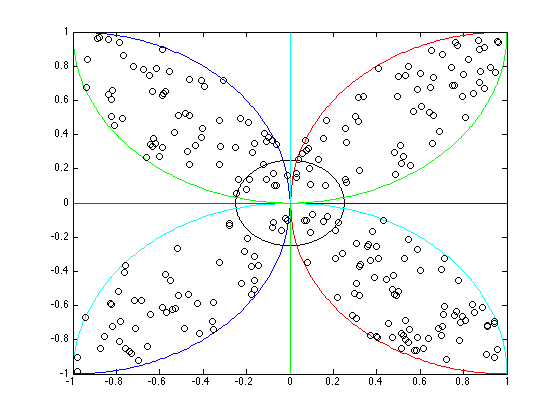
\includegraphics[width=0.8\textwidth]{q8_1.png}
\caption{Desenho das regioes de interesse.}
\label{fig:q8_1}
\end{figure}

A rede foi treinada utilizando a \emph{toolbox} do MATLAB, com o m\'etodo $newsom$, com uma arquitetura 10x10 uniformimente distribuida. Com 500 pontos gerados e 200 itera\c{c}\~oes, tem-se:

\begin{figure}
\centering
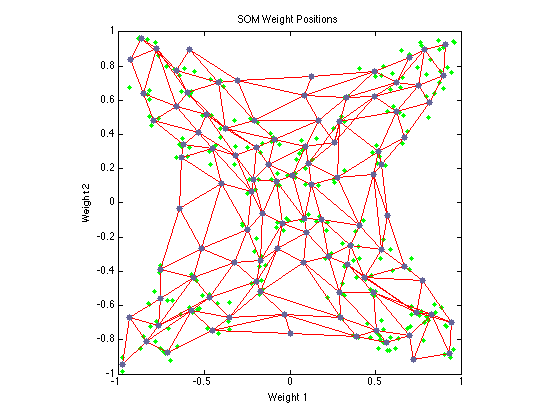
\includegraphics[width=0.8\textwidth]{q8_2.png}
\caption{Resultado da rede.}
\label{fig:q8_2}
\end{figure}

\begin{figure}
\centering
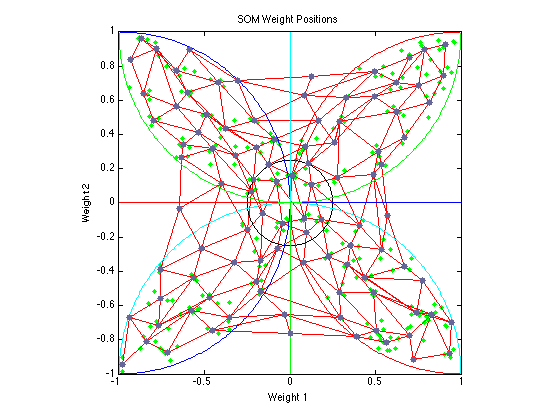
\includegraphics[width=0.8\textwidth]{q8_3.png}
\caption{Resultado da rede com as regioes.}
\label{fig:q8_3}
\end{figure}

As especifica\c{c}\~oes definidas para a execu\c{c}\~ao do treinamento com o algoritmo implementado s\~ao as seguintes: 

Nº de neur\^onios: 100 \\
Nº de \'epocas: 500 \\
Taxa de aprendizagem constante: 0,1 \\
Nº de entradas: 2 \\
Desvio padr\~ao constante: 0,05 \\

Foi implementado o mesmo algoritmo SOM j\'a implementado para classificar os dados destacados em amarelo pertencentes as quatro classes da figura \ref{fig:q8_4}.
Os pesos (círculos vermelhos) e os dados de treinamento (asteriscos azuis) das classes mencionadas acima foram gerados aleatoriamente e normalizados, figura \ref{fig:q8_5}.

\begin{figure}
\centering
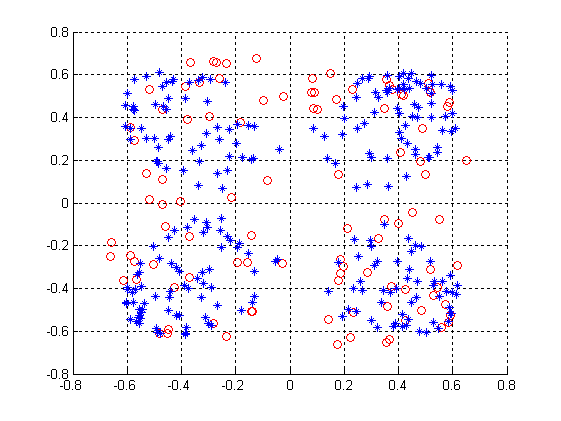
\includegraphics[width=0.8\textwidth]{q8_4.png}
\caption{Inicializa\c{c}\~oes dos dados de treinamento e dos pesos.}
\label{fig:q8_4}
\end{figure}

Ap\'os o treinamento, \'e poss\'ivel notar na figura \ref{fig:q8_5} que os pesos da maioria dos neur\^onios se deslocaram para a regi\~ao dos dados de treinamento, ocorrendo poucos erros.

\begin{figure}
\centering
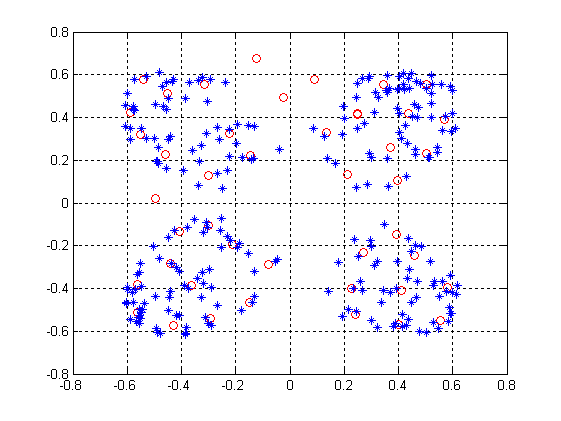
\includegraphics[width=0.8\textwidth]{q8_5.png}
\caption{Resultado da rede SOM treinada que foi implementada.}
\label{fig:q8_5}
\end{figure}

\newpage

\item Pesquise e apresente o formalismo do algoritmo K-means por lote. \\ 

%RESOLU\c{C}\~AO: \\

\item Pesquise e apresente o formalismo do algoritmo SOM por lote. \\

RESOLU\c{C}\~AO: \\

Os algoritmos de particionamento visam subdividir os dados de entrada em n\'umeros fixos de grupos pr\'e-definido e otimizar fun\c{c}\~oes crit\'erios de adequa\c{c}\~ao. Os mais populares s\~ao: K-means e Fuzzy C-means.

O Mapa Auto-Organiz\'avel de Kohonen (SOM) [Kohonen 1995] \'e uma rede neural n\~ao-supervisionada de aprendizado competitivo que possui propriedades de agrupamento e de visualiza\c{c}\~ao. Diferente do K-means, a rede SOM usa um conjunto de intera\c{c}\~oes de vizinhan\c{c}a para aproximar a intera\c{c}\~ao lateral neural e descobrir a estrutura topol\'ogica escondida nos dados, e al\'em do vetor que obteve o melhor valor de similaridade (o vencedor), seus vizinhos tamb\'em s\~ao atualizados, resultando em regi\~oes nas quais neur\^onios em uma mesma vizinhan\c{c}a sejam bastante similares. Tal m\'etodo tamb\'em pode ser considerado como um algoritmo que mapeia dados de alta dimensionalidade espacial, $R^p$, em um espa\c{c}o de dimensionalidade reduzida, geralmente 1D, 2D ou 3D, chamado mapa. Essa proje\c{c}\~ao permite a parti\c{c}\~ao das entradas em grupos ”similares” enquanto preserva sua topologia.

Considerando o algoritmo de mapa auto-organiz\'avel por lote introduzido por [F. Badran and Thiria 2005]. Seja $E = {1,...,n}$ o conjunto de entradas, onde cada entrada $x_{i} = (x_{i1}, ..., x_{ip}) (i = 1, ..., n)$ pertence a $R^p$. Cada neur\^onio do mapa \'e representado por um prot\'otipo $w_{c} = (w_{c1}, ..., w_{cp}) (c = 1, ..., m)$ que tamb\'em pertence a $R_{p}$.

O algoritmo SOM de treinamento por lote [F. Badran and Thiria 2005] \'e um algoritmo iterativo de duas etapas (afeta\c{c}\~ao e representa\c{c}\~ao, discutidos em seguida) onde todo o conjunto de dados (E) \'e apresentado ao mapa antes de algum ajuste ser feito. O algoritmo SOM por lote minimiza a seguinte fun\c{c}\~ao objetiva:

\begin{equation}
J = \sum_{i=1}^{n} \sum_{r=1}^{m} K^{T} (\delta(f^{T}(x_{i}),r))d^{2}(x_{i},w_{r})
\end{equation}

onde $f$ \'e a fun\c{c}\~ao de aloca\c{c}\~ao e $f(x_{i})$ representa o neur\^onio do mapa correspondente ao indiv\'iduo $x_{i}$, e $\delta(f(x_{i})$, $r$ \'e a dist\^ancia entre o neur\^onio $r$ do mapa e o neur\^onio correspondente a $x_{i}$. Assim, $K^T$, que \'e parametrizada por $T$ (onde $T$ representa a temperatura), \'e a fun\c{c}\~ao kernel de vizinhança que define a regi\~ao de influ\^encia de cada neur\^onio $r$. Essa fun\c{c}\~ao objetivo \'e minimizada apenas para um valor de $T$ fixo.

Essa fun\c{c}\~ao de custo \'e uma extens\~ao da fun\c{c}\~ao de custo do K-means, onde a dist\^ancia euclidiana \'e substitu\'ida por:

\begin{equation}
d^{T}(x_{i}, w_{f}(x_{i})) = \sum_{r=1}^{m} K^{T} (\delta(f^{T}(x_{i}),r))d^{2}(x_{i},w_{r})
\end{equation}

onde

\begin{equation}
d^{2}(x_{i},w_{r}) = \sum_{j=1}^{p} (x_{ij} - w_{rj})^2
\end{equation}

\'e a dist\^ancia euclidiana. Essa dist\^ancia generalizada \'e uma soma ponderada das dist\^ancias euclidianas entre $x_{i}$ e todos os vetores de refer\^encia da vizinhan\c{c}a do neur\^onio $f(x_{i})$. Todos os neur\^onios do mapa s\~ao levados em considera\c{c}\~ao.

Quanto $T$ \'e fixo, a minimiza\c{c}\~ao de $J$ \'e realizada em duas etapas iterativas: uma afeta\c{c}\~ao e uma representa\c{c}\~ao.
Durante a etapa de afeta\c{c}\~ao, os vetores de refer\^encia (prot\'otipos) permanecem fixos. A fun\c{c}\~ao de custo $J$ \'e minimizada em rela\c{c}\~ao \`a fun\c{c}\~ao de aloca\c{c}\~ao e cada indiv\'iduo $x_{i}$ \'e assinalado ao seu neur\^onio mais pr\'oximo:

\begin{equation} \label{eq:c}
c = f^{T}(x_{i}) = \text{arg} min_{1\leq r \leq m} d^{T}(x_{i}, w_{r})
\end{equation}

Durante a etapa de representa\c{c}\~ao, a fun\c{c}\~ao de aloca\c{c}\~ao \'e fixada. A fun\c{c}\~ao de custo $J$ \'e minimizada em rela\c{c}\~ao aos prot\'otipos. O prot\'otipo $w_{c}$ \'e atualizado para cada neur\^onio de acordo com:

\begin{equation} \label{eq:w}
w_{c} = \frac{ \sum_{i=1}^{n} K^{T} (\delta(fˆ{T}(x_{i},c))x_{i} }{ \sum_{i=1}^{n} K^{T} (\delta(f^{T}(x_{i},c)) }
\end{equation}

O algoritmo de mapa auto-organiz\'avel por lote (BSOM) [F. Badran and Thiria 2005] pode ser resumido como:
\begin{enumerate}[1)]
\item Inicializa\c{c}\~ao \\
Fixe o n\'umero m de neur\^onios (grupos); \\
Fixe $\delta$; Fixe a fun\c{c}\~ao de kernel $K^T$; \\
Fixe o n\'umero de itera\c{c}\~oes Niter; \\
Fixe $T_{min}$, $T_{max}$; Fa\c{c}a $T \gets T_{max}$; Fa\c{c}a $t \gets 0$; \\
Selecione aleatoriamente m prot\'otipos distintos $w_{c}(0) \text{,} E (c = 1;...,m)$; \\
Inicialize o mapa $L(m;W^{0})$, onde $W^{0} = (w_{1}^{(0)}, \cdots, w_{m}^{(0)} )$; \\
Afete cada objeto $x_{i}$ ao neur\^onio mais pr\'oximo (grupo) do mesmo de acordo com
a equação \ref{eq:c}. \\

\item Etapa 1: Representa\c{c}\~ao. \\
Fa\c{c}a $T = T_{max} (\frac{T_{min}}{T_{max}})^{ \frac{t}{N_{iter} - 1} }$ \\
Mantenha a fun\c{c}\~ao de aloca\c{c}\~ao fixa; \\
Calcule os prot\'otipos $w_{c}^{(t)} (c = 1, ..., m)$ de acordo com a equa\c{c}\~ao \ref{eq:w}; \\

\item Etapa 2: Afeta\c{c}\~ao. \\
Os prot\'otipos $w_{c}^{(t)} (c = 1, ..., m)$ s\~ao fixados. Afete cada indiv\'iduo $x_{i} (i = 1, ..., n)$ ao neur\^onio mais pr\'oximo do mesmo de acordo com a equa\c{c}\~ao \ref{eq:c}; \\

\item Crit\'erio de parada. \\
se $T = T_{min}$, pare; caso contr\'ario, fa\c{c}a $t = t + 1$ e v\'a para o passo 2 (Etapa 1).\\
\end{enumerate}

\end{enumerate}

\newpage

\begin{center}
Trabalhos
\end{center}

\begin{enumerate}[1.]
\item Pesquise e apresente um trabalho sobre a reconstru\c{c}\~ao tridimensional usando a rede SOM e a rede Neuro-GAS. \\

\item Pesquise e apresente um trabalho sobre Neurofuzzy. \\
	
\end{enumerate}

Data de entrega: 23/05/2013 \\

A entrega e apresenta\c{c}\~ao dos trabalhos correspondem a um processo de avalia\c{c}\~ao. Portanto a presen\c{c}a \'e obrigat\'orio. \\

Os trabalhos e a lista podem ser feito em grupo de at\'e tr\^es componentes. \\

Na apresenta\c{c}\~ao os componentes ser\~ao submetidos a questionamentos sobre a solu\c{c}\~ao da lista e o desenvolvimento dos trabalhos. \\

\newpage

\begin{center}
Desenvolvimento da Pesquisa
\end{center}

Pesquise e apresente um trabalho sobre Neurofuzzy. \\

Os sistemas fuzzy s\~ao implementados a partir do conhecimento emp\'irico fornecido por especialistas, j\'a as Redes Neurais Artificiais necessitam  do conhecimento impl\'icito extra\'ido de um conjunto de dados. Visando aproveitar essas duas caracter\'isticas inerentes a cada uma dessas t\'ecnicas, os pesquisadores desenvolveram uma t\'ecnicas para gerar um modelo h\'ibrido e assim, minimizar as defici\^encias.
Os sistemas h\'ibridos s\~ao a combina\c{c}\~ao de duas ou mais t\'ecnicas, em que, uma pode ser aplicada para melhorar as defici\^encias de outra.  Assim, os Sistemas Neuro-Fuzzy (SNF) \'e um tipo de sistema h\'ibrido incorporado pela combina\c{c}\~ao entre os Sistemas Fuzzy e as Redes Neurais Artificiais.

Os SNF \'e um Sistema de infer\^encia Fuzzy, cujos par\^ametros  s\~ao ajustados atrav\'es de algoritmos de aprendizagem de redes neurais, como ilustrado na figura \ref{fig:f_1}.

\begin{figure}[h]
\centering
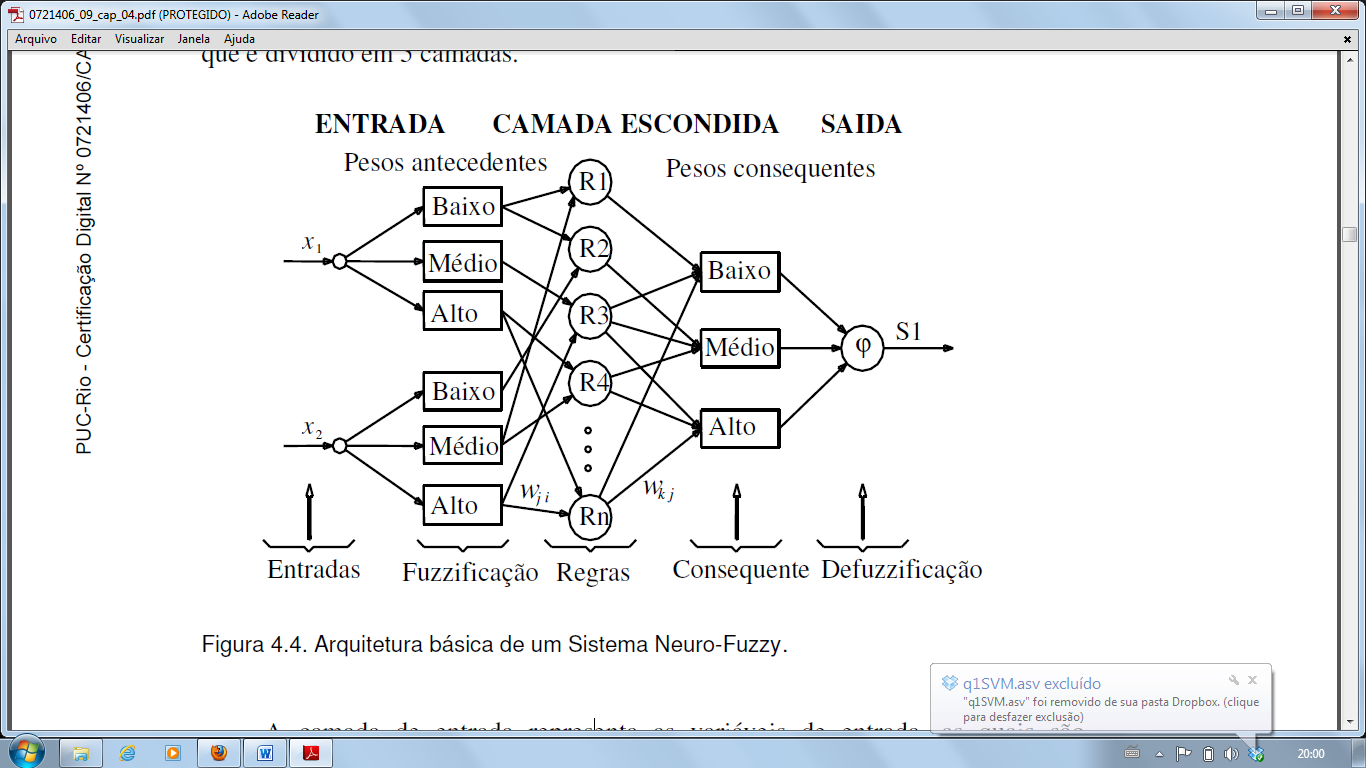
\includegraphics[trim=4cm 5cm 4cm 4cm, clip=true, width=0.8\textwidth]{f_1.png}
\caption{Sistema Fuzzy.}
\label{fig:f_1}
\end{figure}

\begin{figure}[h]
\centering
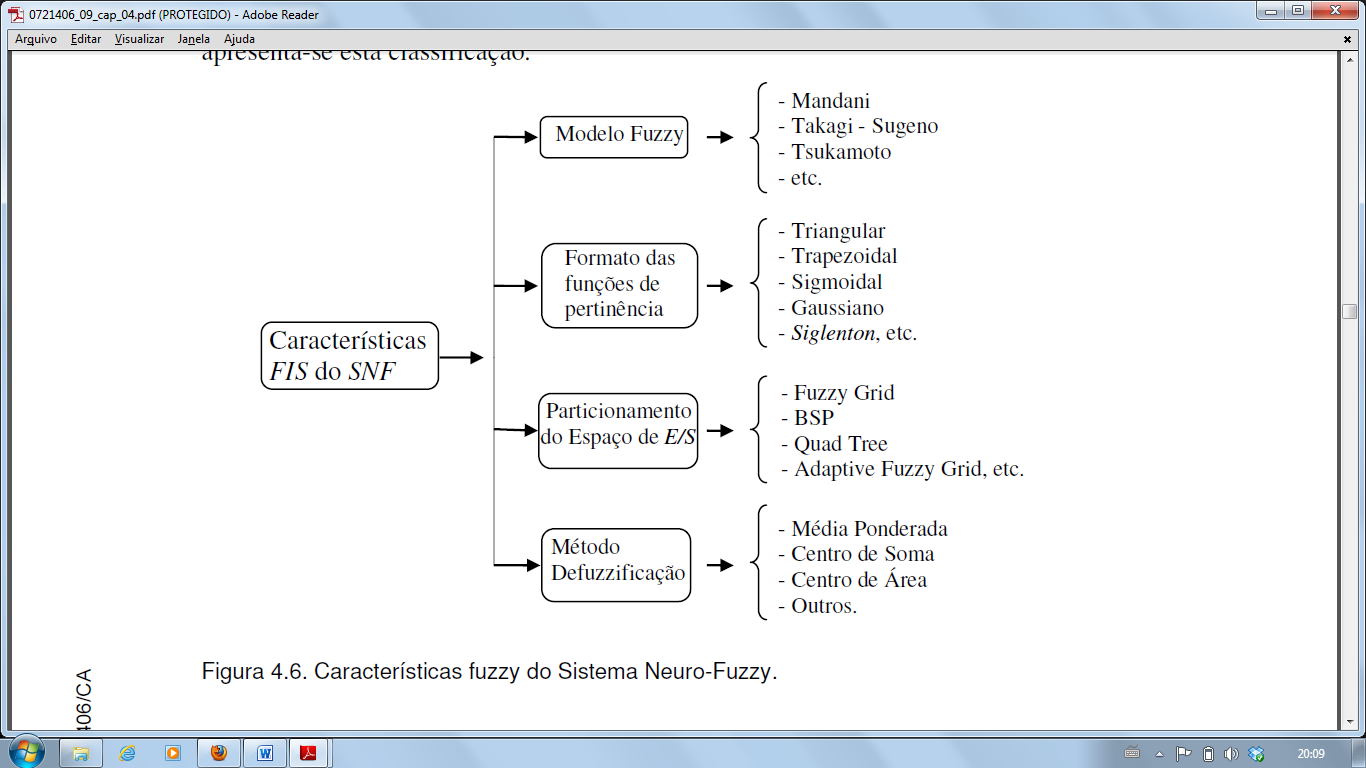
\includegraphics[trim=4cm 5cm 4cm 4cm, clip=true, width=1\textwidth]{f_2.png}
\caption{Caracteristicas Fuzzy.}
\label{fig:f_2}
\end{figure}

As caracter\'isticas Fuzzy do SNF s\~ao agrupadas em 4 Sub-classes demonstradas no esquema abaixo.

As caracter\'isticas neurais do SNF est\~ao divididas em tr\^es sub-classes apresentadas abaixo.

Alguns dos principais modelos de SNF s\~ao: \\
Adaptative Network based Fuzzy Inference Systems (ANFIS) \\
Neuro Fuzzy Classification (NEFCLASS) \\
Fuzzy Self-organized Map (FSOM) \\

As vantagens da utiliza\c{c}\~ao de SNF s\~ao:\\
Grande potencial para aplica\c{c}\~oes que combinam conhecimento qualitativo com robustez \\
Possuem interfaces de alto n\'ivel, de r\'apida computa\c{c}\~ao e programa\c{c}\~ao amig\'avel. Apresentando conveni\^encia para a extra\c{c}\~ao de conhecimentos atrav\'es do aprendizado. \\
Aus\^encia da necessidade do conhecimento pr\'evio do processo e melhora no processamento de ru\'idos dos dados. \\
Capacidade de auto-aprendizado, auto-organiza\c{c}\~ao e auto-direcionamento. \\

Como desvantagens o SNF tem: \\
N\'umero de entradas reduzidos \\
Limita\c{c}\~ao da constru\c{c}\~ao de sua pr\'opria estrutura, limitados pelo elevado n\'umero de regras. \\

\end{document}